\section{Methodology}\label{sec:methodology}

\subsection{Application as Finite State Machine with centralized state}\label{sec:central_state}
Lo sviluppo del progetto si \`e focalizzato sull'individuazione di una struttura gerarchica di oggetti Javascript in grado di rappresentare in modo esaustivo l'insieme delle componenti presenti sulla planimetria. L'intero stato dell'applicazione viene descritto da una \textbf{struttura ad albero immutabile} di cui viene mantenuto un riferimento al nodo radice. Ciascuna modifica atomica corporta: (i) La creazione di un nuovo stato \texttt{s'} identico al precedente stato \texttt{s}; (ii) L'applicazione delle modifiche allo stato \texttt{s'}; (iii) La modifica del puntatore che rappresenta lo stato corrente da \texttt{s} ad \texttt{s'}. Dal punto di vista della gestione della memoria questo meccanismo richiederebbe un importante dispendio di risorse. Per evitare ci\`o l'implementazione \textbf{Immutable.js}~\footnote{https://facebook.github.io/immutable-js/} realizzata da Facebook, adotta dei meccanismi che simulano il principio di immutabilit\`a evitando la copia in profondit\`a della memoria  (deep clone).

La gestione centralizzata dello stato permette lo sviluppo di funzionalità che hanno come unico obiettivo la creazione di un nuovo stato coerente con la modifica richiesta, senza la necessità di agire sull'interfaccia o su qualsiasi altro componente in esecuzione. L'adeguamento dell'interfaccia grafica al nuovo stato viene effettuato secondo i meccanismi descritti nella sezione~\ref{sec:ui_components}.

Memorizzando la storia di tutti gli stati generati dall'applicazione e sfruttando le garanzie offerte dall'immutabilità si può effettuare, in qualsiasi momento, un'operazione di redo ad un vecchio stato attraverso la sostituzione dello stato corrente con uno qualsiasi tra quelli passati.

Per dominare la complessit\`a dell'applicazione l'intero sistema \`e stato modellato su una macchina a stati. Sfruttando il modello basato su azioni e reducer messo a disposizione dal \textbf{pattern unidirectional data flow} \`e stato individuato un grafo che rappresenta le possibili evoluzioni dello stato dell'applicazione. Ogni nodo corrisponde ad una \textbf{modalit\`a}, ogni arco corrisponde alle possibili azioni che è possibile intraprendere a partire da quel punto. A seconda della modalit\`a gli eventi del browser, come ad esempio \texttt{click} o \texttt{mousemove}, vengono mappati sulle azioni. Un estratto della macchina a stati \`e presente in figura~\ref{fig_uc_draw_wall}.

La gestione dello stato centralizzato e la gestione della logica applicata realizzata  attraverso la modellazione di una macchina a stati è stata possibile sfruttando l'implementazione messa a disposizione dalla libreria \textbf{Redux.js}~\footnote{http://redux.js.org/}.


\begin{figure}[!t]
\centering
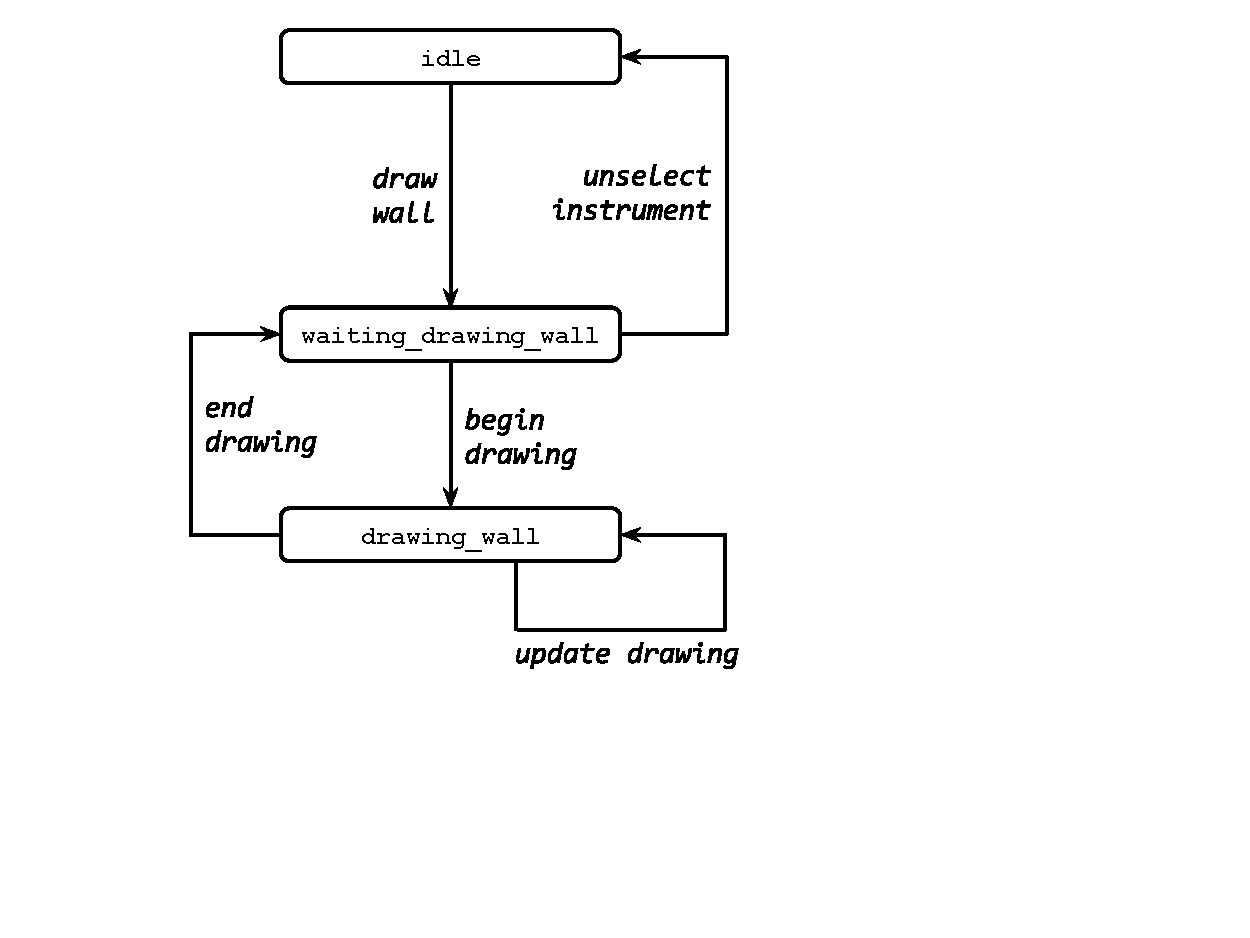
\includegraphics[width=0.6\linewidth]{contents/images/uc_draw_wall}

\caption{Sottografo della macchina a stati che rappresenta la creazione di un muro. (i) Nodo \texttt{idle}: modalit\'a d'attesa dell'applicazione. Non è stata ancora intrapresa nessuna operazione. (ii) Nodo \texttt{waiting\_drawing\_wall}: l'utente ha selezionato lo strumento disegno muro, ma non ha ancora iniziato il disegno. (iii) Nodo \texttt{drawing\_wall}: l'utente ha posizionato il punto di inizio del muro.}
\label{fig_uc_draw_wall}
\end{figure}


\subsection{Collaboration}  

Diamo ora un cenno sull'architettura scelta per permettere la collaborazione tra utenti diversi nella modellazione dello stesso edificio. In letteratura esistono diverse tecniche per realizzare una piattaforma di collaborazione tra utenti remoti. Un esempio \`e dato da~\cite{Ellis:1989:CCG:66926.66963} dove viene introdotta la tecnologia \textbf{Operational Transformation}. Con questa tecnica un gruppo di nodi si scambia messaggi senza un \textit{punto di controllo centrale} basandosi su due propriet\`a: (i) you can transform changes relative to other changes and (ii) there is no matter in which order concurrent changes are applied, you end up with the same document.\\

Tuttavia, la gestione centralizzata dello stato ed in generale l'applicazione del pattern uniflow ci hanno suggerito di adottare una diversa metodologia per l'introduzione della collaborazione. In accordo con questi principi abbiamo preferito una \textbf{centralized topology} per la comunicazione tra nodi. Con questo approccio lo stato viene condiviso da pi\`u applicazioni sfruttando meccanismi di comunicazione per la sincronizzazione. Questo tipo di topologia ci ha suggerito di evitare routine di sincronizzazione peer-to-peer, anche per non affrontare problemi di implementazione dovuti all'infrastruttura di rete (ad esempio a causa del NAT) comuni nei sistemi di questo tipo. In ogni caso, questo approccio non influisce sulla natura serverless dell'architettura in quanto i servizi di comunicazione sono esterni (in particolare nella nostra applicazione abbiamo usato firebase come meccanismo per lo scambio di dati centralizzato).

\subsection{Building elements}\label{building_elements}

L'insieme degli elementi che \`e possibile inserire all'interno della planimetria vengono gestiti in un \textbf{catalogo}, strutturato in categorie.
La categorizzazione individua un insieme di casi d'uso con cui l'utente pu\`o interagire.\\\\
\textbf{Walls}, rientrano in questa categoria tutti i tipi di muro (perimetrali, interni, portanti). La creazione avviene specificando il punto di inizio e fine dell'elemento. La rappresentazione interna viene ricondotta a quella di un grafo in cui: i \textbf{nodi} corrispondono ai punti geometrici in cui si intersecano pi\`u muri e hanno delle coordinate che li collocano nello spazio; gli \textbf{archi} corrispondono al muro. Questa rappresentazione garantisce inoltre un’efficace risposta alle operazioni di drag and drop sui muri: ogni spostamento viene applicato attraverso la modifica della posizione dei nodi comportando, oltre allo spostamento del muro richiesto, un riposizionamento di tutti i muri adiacenti.\\\\
\textbf{Openings}, rientrano in questa categoria gli elementi che bucano i muri come porte, finestre e archi. La creazione viene effettuata attraverso uno snap sui muri precedentemente creati. La rappresentazione interna associa ciascuna apertura con il muro di riferimento, creando un legame tra le due componenti.\\\\
\textbf{Areas}, rientrano in questa categoria i pavimenti. La creazione viene effettuata automaticamente attraverso un'analisi del grafo composto dai muri. L'algoritmo individuato si compone delle seguenti fasi: (i) Ricerca delle componenti biconnesse attraverso l'applicazione dell'algoritmo Hopcroft-Tarjan~(vedi \cite{Hopcroft:1973:AEA:362248.362272}); 
(ii) Rimozione degli archi che non appartengono alle componenti biconnesse; 
(iii) Individuazione di tutti i cicli attraverso una doppia visita degli archi ordinata rispetto ad un angolo;
(iv) Individuazione dei cicli massimali, corrispondenti ai cicli che coinvolgono tutti gli archi perimetrali del grafo attraverso la Gauss's area formula;
(v) Rimozione dei cicli massimali.\\\\
\textbf{Objects}, rientrano in questa categoria tutti gli oggetti posizionabili sulle aree. L'utente pu\`o agire sulla disposizione sia in termini di posizione che rotazione.\\

\subsection{UI components}\label{sec:ui_components}

L'intera applicazione \`e stata progettata in maniera modulare, rifacendosi ai principi di \textbf{SOLID programming} in modo che sia espandibile. Dal punto di vista web il pattern di riferimento \`e stato quello dei \textbf{web components}, sfruttando l'implementazione di \textbf{React.js}~\footnote{https://github.com/facebook/react} realizzata da Facebook. L'idea di base \`e quello di definire l'applicazione frontend come una collezione di componenti, che vengono renderizzati in modo diverso a seconda dei valori assegnati allo stato. In figura~\ref{fig_ui} abbiamo un esempio di applicazione di questa tecnologia. \\

\begin{figure}[h]
\centering
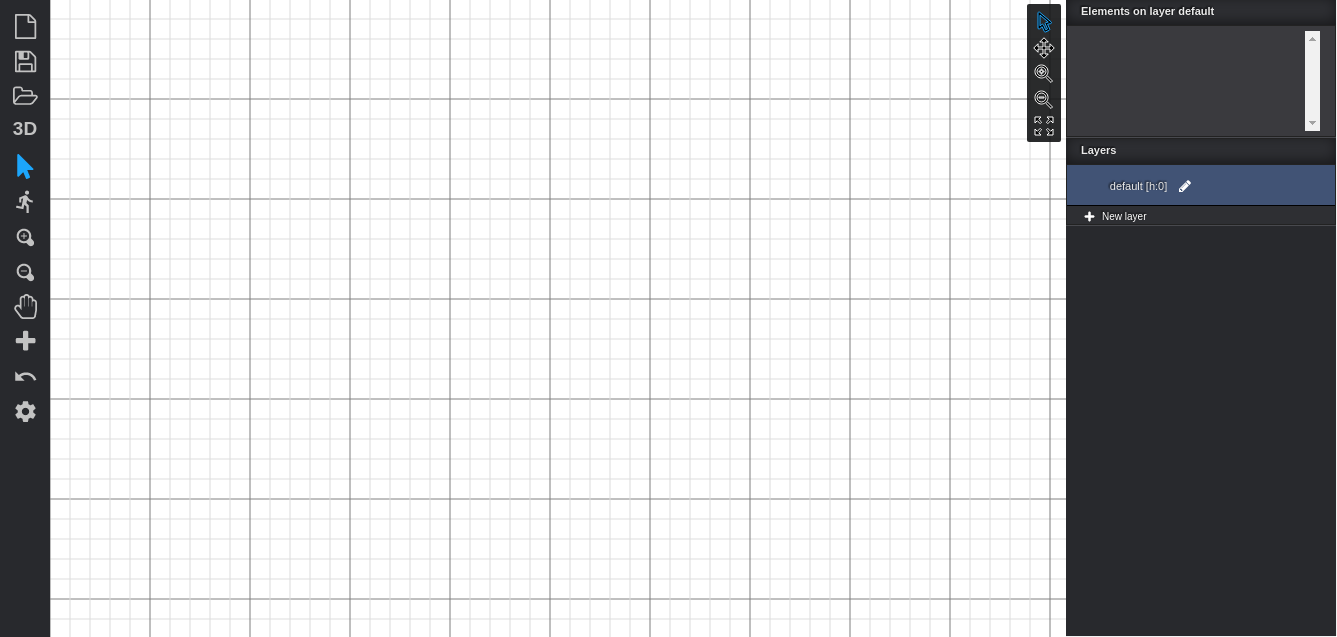
\includegraphics[width=0.65\linewidth]{contents/images/ui}\\
\caption{The user interface of the application with the most interesting components: the toolbar (where every button is another component), the sidebar and the 2D viewer}
\label{fig_ui}
\end{figure}

Entrando nel dettaglio, una classe interessante di componenti che sono delegati alla rappresentazione delle propriet\`a dello stato sono i \textbf{viewers}. Esempi sono i visualizzatori per il 2D e per il 3D. In generale, la struttura a componenti permette di definire una qualunque visualizzazione dello stato (ad esempio in forma tabellare) inserendo un nuovo componente.\\

La struttura dei visualizzatori \`e schematizzata nella figura~\ref{fig_viewers}, dove siamo in grado di identificare tre macro blocchi. Il primo \`e il catalogo, che come abbiamo visto nel paragrafo \ref{building_elements} contiene tutti i building elements del sistema e le loro properiet\`a. Il secondo \`e il core vero e proprio e si occupa della gestione dello stato e contiene le funzionalit\`a di disegno. Questo comunica con il catalogo prendendo le propriet\`a dei building elements. Infine abbiamo i visualizzatori veri e propri, che vengono scelti in base alla modalit\`a corrente dello stato (vedi la sezione~\ref{sec:central_state}). Al momento sono stati implementati i visualizzatori 2D e 3D (vedi la figura~\ref{fig_viewer}).\\\\
\textbf{2D Viewer}. This viewer creates a 2D view of the building model. Dato lo stato, \`e in grado di sfruttare il \textbf{Virtual DOM}~\footnote{https://facebook.github.io/react/docs/optimizing-performance.html, https://github.com/Matt-Esch/virtual-dom}, nell'implementazione di React.js, per aggiornare solo le parti che vengono modificate evitando aggiornamenti globali continui.\\\\
\textbf{3D Viewer}. Sfrutta la libreria di modellazione per WebGL \textbf{Three.js}~\footnote{https://threejs.org/} per creare una vista 3D del building model. Per evitare di dover continuamente ricreare l'intero modello quando cambiano porzioni dello stato, \`e stato implementato un sistema di \textit{diff} e \textit{patch} dello stato standardizzato in~\cite{rfc6902}. In pratica \`e stata creata una struttura parallela che mappa gli oggetti di Three.js con i relativi building elements memorizzati nello stato. Ogni volta che viene lanciata un'azione Redux.js, viene calcolata la diff tra il vecchio stato e quello nuovo e si ricreano solo gli oggetti che sono stati modificati. In particolare possiamo avere tre possibili \textit{operations}: (i) \textbf{add}, (ii) \textbf{replace} and (iii) \textbf{remove}. For every operation, viene determinato un diverso tipo di comportamento in base al particolare building element cambiato, coinvolgendo eventualmente building elements correlati



\begin{figure}[htb]
\centering
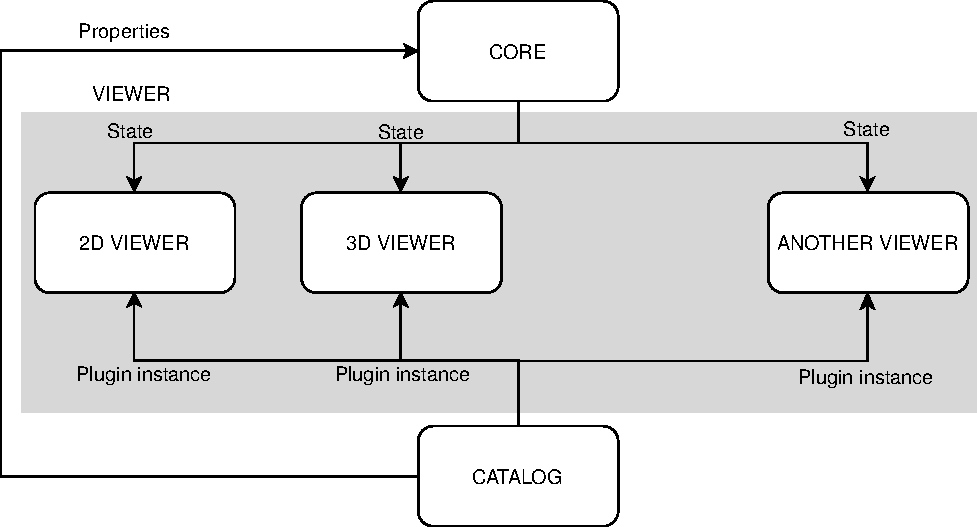
\includegraphics[width=\linewidth]{contents/images/diagramma-visualizzatori}

\caption{The architectural schema for the viewers. Here we can see that the core can instanziate several different viewers giving them the state for the representation}
\label{fig_viewers}
\end{figure}

\begin{figure}[htb]
\centering
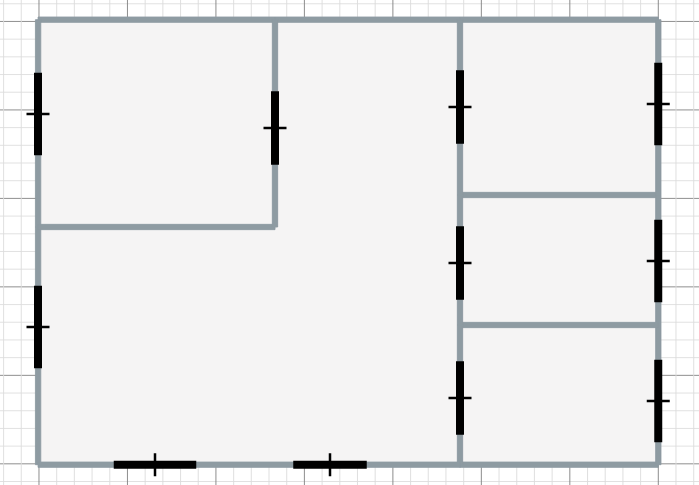
\includegraphics[width=0.45\linewidth]{contents/images/2d-viewer}
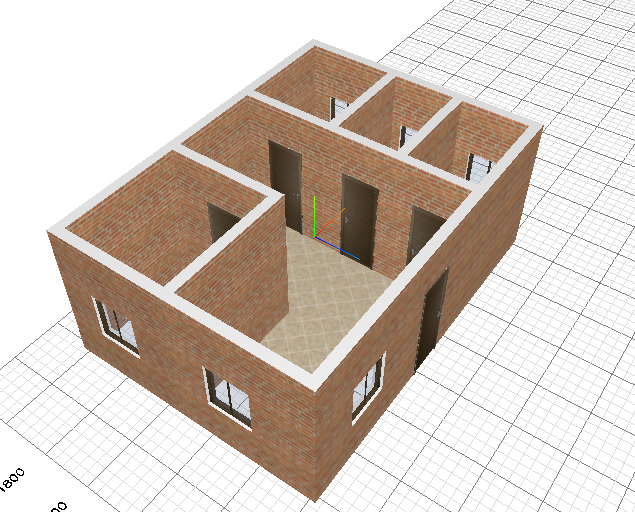
\includegraphics[width=0.45\linewidth]{contents/images/3d-viewer}
\caption{The 2D and 3D viewers for the state}
\label{fig_viewer}
\end{figure}

\subsection{Architettura serverless}
Una tra le sfide che ha caratterizzato il progetto \`e l'utilizzo di un approccio serverless. L'intera applicazione viene eseguita all'interno del browser, ottenendo i vantaggi di: (i) evitare all'utilizzatore complicate installazioni del sistema o procedure di aggiornamento; (ii) fornire un livello di astrazione tale da rendere l'ambiente compatibile su diverse macchine e su diversi sistemi operativi; (iii) abilitare un rilascio di nuove versioni centralizzato, in grado di raggiungere tutti gli utenti contemporanemante; (iv) eliminare il punto di concentramento del calcolo in quanto questo rimane confinato sulla macchina dell'utente.
Per permettere la generazione di elementi architetturali complessi il sistema \`e in grado inoltre di sfruttare dei worker di tipo FaaS (Function as a Service) demandando l'onerosa generazione delle geometrie 3D necessarie alla visualizzazione. Nella figura~\ref{fig_serverless} c'\`e uno schema dell'architettura dell'applicazione
\begin{figure}[htb]
\centering
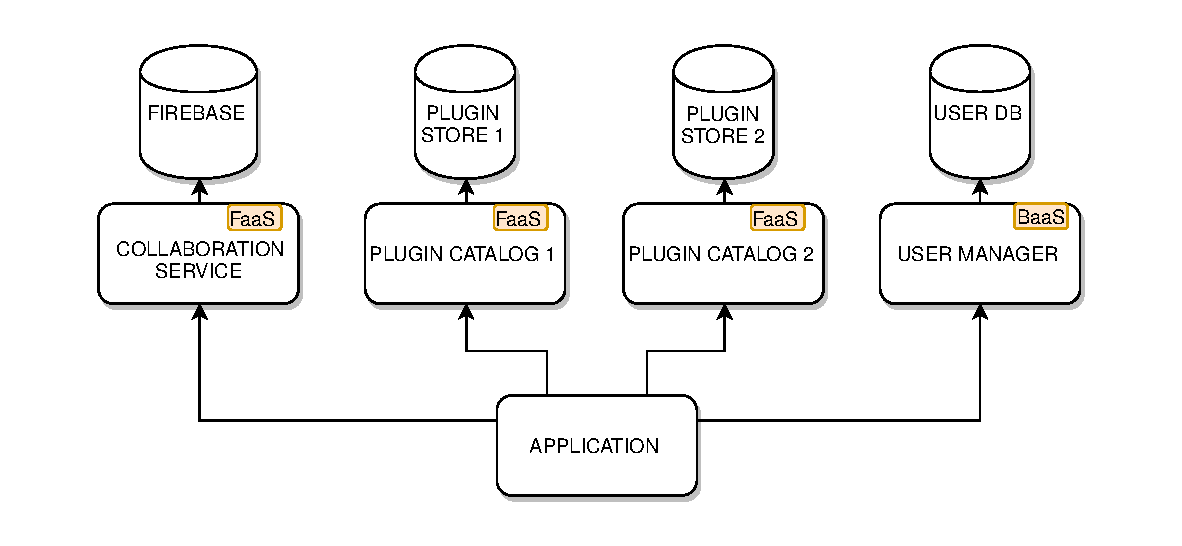
\includegraphics[width=\linewidth]{contents/images/serverless-diagram}

\caption{The serverless architecture for our application. We can recognize the collaboration component, based on firebase. We can also see the FAAS container for the plugin catalog which is linked with a BAAS component for plugins generated on server with other modeling software. We can also manage an optional user login to the system, with another BAAS. Notice that the core application is entirely run on front end side}
\label{fig_serverless}
\end{figure}